%% For double-blind review submission
\documentclass[acmlarge,review,anonymous]{acmart}\settopmatter{printfolios=true}
%% For single-blind review submission
%\documentclass[acmlarge,review]{acmart}\settopmatter{printfolios=true}
%% For final camera-ready submission
%\documentclass[acmlarge]{acmart}\settopmatter{}

%% Note: Authors migrating a paper from PACMPL format to traditional
%% SIGPLAN proceedings format should change 'acmlarge' to
%% 'sigplan,10pt'.


%% Some recommended packages.
\usepackage{mathtools}
\usepackage{mathpartir}
\usepackage{fullpage}
\usepackage{ifpdf}
\usepackage{graphicx}
%\usepackage[usenames,dvipsnames]{color}
\usepackage{subcaption}
\usepackage{stmaryrd}
%\usepackage[numbers]{natbib}
\usepackage{amsthm}
\usepackage{listings}          % format code
\usepackage{xspace}

% Math mode
%-----------
\newenvironment{nop}{}{}
\newenvironment{smathpar}{
\begin{nop}\small\begin{mathpar}}{
\end{mathpar}\end{nop}\ignorespacesafterend}

% Name
%-----
\newcommand{\name}{{\sf DaLi}\xspace}

% Formatting
%---------
\newcommand{\C}[1]{\code{#1}}
\newcommand{\tuplee}[1]{\langle #1 \rangle}
\newcommand*{\rom}[1]{\expandafter\romannumeral #1}

% Formatting commands
% -------------------
\newcommand{\code}[1]{\,{\tt #1}\,}
\newcommand{\spc}[0]{\quad}
\newcommand{\ALT}{~\mid~}
\newcommand{\rel}[1]{{R}_{\mathit{#1}}}
\newcommand{\conj}{~\wedge~}
\newcommand{\disj}{~\vee~}
\newcommand{\rulelabel}[1]{\textrm{\sc {#1}}}
\newcommand{\ilrulelabel}[1]{{\sc #1}}
\newcommand{\RULE}[2]{\frac{\begin{array}{c}#1\end{array}}
                           {\begin{array}{c}#2\end{array}}}
\newcommand{\denot}[1]{\llbracket #1 \rrbracket}
\newcommand{\bind}{>\!\!>\!\!=}
\newcommand{\coloneqq}{::=}
\newcommand{\stepsto}{\longrightarrow}
\newcommand{\return}[1]{\C{return}\;#1}
\newcommand{\run}[2]{\C{run}\;#1\;#2}
\newcommand{\fork}[1]{\C{fork}\;#1}
\newcommand{\push}[1]{\C{push}\;#1}
\newcommand{\pull}{\C{pull}}
\newcommand{\semsucceq}{\succeq_{\circ}}
\newcommand{\sempreceq}{\preceq_{\circ}}
\newcommand{\under}[2]{#1\,\vdash\,#2}
\newcommand{\mbleto}{\rightsquigarrow_m}

% New colors
%------------
\definecolor{Bittersweet}{rgb}{1.0, 0.44, 0.37}

% Listings Code
%---------------
\newcommand{\lstml}{
\lstset{ %
language=ML, % choose the language of the code
basicstyle=\small\ttfamily,       % the size of the fonts that are used for the code
keywordstyle=\color{Bittersweet},
% numbers=left,                   % where to put the line-numbers
numberstyle=\tiny,      % the size of the fonts that are used for the line-numbers
stepnumber=1,                   % the step between two line-numbers. If it is 1 each line will be numbered
numbersep=5pt,                  % how far the line-numbers are from the code
showspaces=false,               % show spaces adding particular underscores
showstringspaces=false,         % underline spaces within strings
showtabs=false,                 % show tabs within strings adding particular underscores
% frame=single,                   % adds a frame around the code
tabsize=2,                      % sets default tabsize to 2 spaces
captionpos=b,                   % sets the caption-position to bottom
breaklines=true,                % sets automatic line breaking
breakatwhitespace=false,        % sets if automatic breaks should only happen at whitespace
commentstyle=\itshape\color{MidnightBlue},
%escapeinside={\%*}{*)},         % if you want to add a comment within your code
morekeywords={module, @@deriving, not, : , /\\}
}}
\lstnewenvironment{ocaml}
    { % \centering
			\lstml
      \lstset{}%
      \csname lst@setfirstlabel\endcsname}
    { %\centering
      \csname lst@savefirstlabel\endcsname}



\makeatletter\if@ACM@journal\makeatother
%% Journal information (used by PACMPL format)
%% Supplied to authors by publisher for camera-ready submission
\acmJournal{PACMPL}
\acmVolume{1}
\acmNumber{1}
\acmArticle{1}
\acmYear{2017}
\acmMonth{1}
\acmDOI{10.1145/nnnnnnn.nnnnnnn}
\startPage{1}
\else\makeatother
%% Conference information (used by SIGPLAN proceedings format)
%% Supplied to authors by publisher for camera-ready submission
\acmConference[PL'17]{ACM SIGPLAN Conference on Programming Languages}{January 01--03, 2017}{New York, NY, USA}
\acmYear{2017}
\acmISBN{978-x-xxxx-xxxx-x/YY/MM}
\acmDOI{10.1145/nnnnnnn.nnnnnnn}
\startPage{1}
\fi


%% Copyright information
%% Supplied to authors (based on authors' rights management selection;
%% see authors.acm.org) by publisher for camera-ready submission
\setcopyright{none}             %% For review submission
%\setcopyright{acmcopyright}
%\setcopyright{acmlicensed}
%\setcopyright{rightsretained}
%\copyrightyear{2017}           %% If different from \acmYear


%% Bibliography style
\bibliographystyle{ACM-Reference-Format}
%% Citation style
%% Note: author/year citations are required for papers published as an
%% issue of PACMPL.
\citestyle{acmauthoryear}   %% For author/year citations



\begin{document}

%% Title information
\title[]{Highly-Available Functional Replicated Datatypes}         %% [Short Title] is optional;
                                        %% when present, will be used in
                                        %% header instead of Full Title.
%\titlenote{with title note}             %% \titlenote is optional;
                                        %% can be repeated if necessary;
                                        %% contents suppressed with 'anonymous'
%\subtitle{Subtitle}                     %% \subtitle is optional
%\subtitlenote{with subtitle note}       %% \subtitlenote is optional;
                                        %% can be repeated if necessary;
                                        %% contents suppressed with 'anonymous'


%% Author information
%% Contents and number of authors suppressed with 'anonymous'.
%% Each author should be introduced by \author, followed by
%% \authornote (optional), \orcid (optional), \affiliation, and
%% \email.
%% An author may have multiple affiliations and/or emails; repeat the
%% appropriate command.
%% Many elements are not rendered, but should be provided for metadata
%% extraction tools.

%% Author with single affiliation.
\author{First1 Last1}
\authornote{with author1 note}          %% \authornote is optional;
                                        %% can be repeated if necessary
\orcid{nnnn-nnnn-nnnn-nnnn}             %% \orcid is optional
\affiliation{
  \position{Position1}
  \department{Department1}              %% \department is recommended
  \institution{Institution1}            %% \institution is required
  \streetaddress{Street1 Address1}
  \city{City1}
  \state{State1}
  \postcode{Post-Code1}
  \country{Country1}
}
\email{first1.last1@inst1.edu}          %% \email is recommended

%% Author with two affiliations and emails.
\author{First2 Last2}
\authornote{with author2 note}          %% \authornote is optional;
                                        %% can be repeated if necessary
\orcid{nnnn-nnnn-nnnn-nnnn}             %% \orcid is optional
\affiliation{
  \position{Position2a}
  \department{Department2a}             %% \department is recommended
  \institution{Institution2a}           %% \institution is required
  \streetaddress{Street2a Address2a}
  \city{City2a}
  \state{State2a}
  \postcode{Post-Code2a}
  \country{Country2a}
}
\email{first2.last2@inst2a.com}         %% \email is recommended
\affiliation{
  \position{Position2b}
  \department{Department2b}             %% \department is recommended
  \institution{Institution2b}           %% \institution is required
  \streetaddress{Street3b Address2b}
  \city{City2b}
  \state{State2b}
  \postcode{Post-Code2b}
  \country{Country2b}
}
\email{first2.last2@inst2b.org}         %% \email is recommended


%% Paper note
%% The \thanks command may be used to create a "paper note" ---
%% similar to a title note or an author note, but not explicitly
%% associated with a particular element.  It will appear immediately
%% above the permission/copyright statement.
%\thanks{with paper note}                %% \thanks is optional
                                        %% can be repeated if necesary
                                        %% contents suppressed with 'anonymous'


%% Abstract
%% Note: \begin{abstract}...\end{abstract} environment must come
%% before \maketitle command
\begin{abstract}
Text of abstract \ldots.
\end{abstract}


%% 2012 ACM Computing Classification System (CSS) concepts
%% Generate at 'http://dl.acm.org/ccs/ccs.cfm'.
\begin{CCSXML}
<ccs2012>
<concept>
<concept_id>10011007.10011006.10011008</concept_id>
<concept_desc>Software and its engineering~General programming languages</concept_desc>
<concept_significance>500</concept_significance>
</concept>
<concept>
<concept_id>10003456.10003457.10003521.10003525</concept_id>
<concept_desc>Social and professional topics~History of programming languages</concept_desc>
<concept_significance>300</concept_significance>
</concept>
</ccs2012>
\end{CCSXML}

\ccsdesc[500]{Software and its engineering~General programming languages}
\ccsdesc[300]{Social and professional topics~History of programming languages}
%% End of generated code


%% Keywords
%% comma separated list
\keywords{keyword1, keyword2, keyword3}  %% \keywords is optional


%% \maketitle
%% Note: \maketitle command must come after title commands, author
%% commands, abstract environment, Computing Classification System
%% environment and commands, and keywords command.
\maketitle


\section{Introduction}
\label{sec:intro}

Real-world distributed programs are challenging to write and maintain
because they often conflate two distinct mechanisms.  The first
concerns the expression of application logic - how do we define
computations that are robust in the presence of distributed
communication among concurrently executing threads of control?  The
second deals with system concerns - how do we express notions of
visibility, replication, and consistency when the nodes participating
in such computations may be geographically distributed and the
networks that connect them unreliable?  To simplify reasoning in such
complicated environments, programming models often make strong
assumptions on the guarantees provided by an implementation (such as
serializability~\cite{Serializability} or strong
consistency~\cite{CDE+12,DNN+15}) that may inadvertently mask,
restrict, or ignore important albeit unpleasant realities (e.g.,
network partitions~\cite{Brewer2000,Gilbert2002}). When unwarranted
assumptions are made, program behavior is often difficult to predict
and verify.  On the other hand, when these features are explicitly
exposed to the programmer, e.g., by requiring that applications be
written in terms of specialized distributed data
structures~\cite{Burckhardt2014,BFL+12,SPB+11} or control
primitives~\cite{Calm}, simplicity, composability, and
ease-of-reasoning can suffer.

To illustrate how these kinds of problems manifest in practice,
consider how we might write a simple counter library (see
Fig.~\ref{fig:counter-adt}).  A \C{Counter} supports two (update)
operations - \C{add} and \C{mult} - that lets a non-negative integer
value be added or multiplied to the counter, resp.  Observe that the
library is written in an idiomatic functional style, with no special
reasoning principles needed to realize desired functionality.  As long
as applications use the library on a single machine, this
implementation behaves as expected.  However, if the library is used
in the context of a more sophisticated application, say one whose
computation is distributed among a collection of machines, its
behavior can become significantly harder to understand.  In
particular, a distributed implementation might wish to
\emph{replicate} the counter state on each node to improve response
time or fault tolerance.  Unfortunately, adding replication doesn't
come for free.  Attempting to update every replicated copy atomically
is problematic in the absence of sophisticated transaction support,
which impose significant performance penalties.  But, without such
heavyweight mechanisms, applying an \C{Add} operation on one node may
not be instanteously witnessed on another, which may be in the process of
simultaneously attempting to perform its own \C{Add} or \C{Mult}
action.  While synchronizing the activities of all nodes to ensure at
most one such operation is performed at a time is impractical,
designating a single node to hold the counter state eschewing
replication altogether (as in a client-server
configuration~\cite{Armstrong}), is also an undesirable solution,
given the sensitivity of such architectures to network partitions and server failures, and
the negative performance impact it incurs in geo-distributed
environments~\cite{Walter}.  Removig coordination altogether by simply
replicating counter state without having any supporting consistency
protocol is an equally infeasible approach.

A method often adopted to address these concerns is to re-define a
datatype's operations to return \emph{effects} instead of
values~\cite{SPB+11,Burckhardt2014}.  An \emph{effect} is a tag that
identifies the operation to be applied uniformly at all replicas to
incorporate the effects of the original
operation. Fig.~\ref{fig:counter-rdt} shows the \C{Counter} library
with operations re-defined to returns effects.  Observe that the
\C{Counter.add x v} operation now returns an \C{Add x} effect, which,
when applied at a replica (see \C{apply} in the figure), adds \C{x} to
the local counter value.  Note, however, that \C{add} and \C{mult} are
not commutative operations - assuming two replicas have the same
initial counter value of 0, applying the effect of adding 3 and then
multiplying 5 on one replica yields 15, while applying the effect of
first multiplying 5 and then adding 3 yields 3 on the other.  Such
scenarios are possible in a distributed system because there are no
coherence guarantees on the order in which effects are received by
different nodes.  Thus, implementations must be carefully written to
take the lack of commutativity into account when defining how effects
are applied at a replica; in the figure, multiplication is expressed
in terms of addition to avoid the kind of undesirable behavior
described above.

In this implementation, all replicas will eventually contain the same
counter value, assuming updates to the counter eventually quiesces.
While transmitting effects provide a low-level operational basis for
handling replicated state, the \emph{ad hoc} nature of the solution
confounds desirable high-level reasoning principles.  Indeed, the
semantic gap between the two versions of the counter, one cognizant of
replication and the other not, breaks backward compatibility with the
original state-based implementation.  Just as significantly, its
non-trivial construction must be developed in different guises for
every distributed data structure used by the application.
\begin{figure}
\begin{subfigure}[b]{0.4\textwidth}
  \begin{ocaml}
    module Counter: sig
      type t
      val add: int -> t -> t
      val mult: int -> t -> t
      val read: t -> int
    end = struct
      type t = int
      let add x v = v + (abs x)
      let mult x v = v * (abs x)
      let read v = v
    end
  \end{ocaml}
\caption{\C{Counter} library in OCaml}
\label{fig:counter-adt}
\end{subfigure}
\begin{subfigure}[b]{0.56\textwidth}
  \begin{ocaml}
    module Counter: sig
      type t
      type eff
      val add: int -> t-> eff
      val mult: int -> t -> eff
      val apply: eff -> t -> t
      val read: t -> int
    end = struct
      type t = int
      type eff = Add of int
      let add x v = Add (abs x)
      let mult x v = Add (v * (abs x - 1))
      let apply (Add x) v = x + v
      let read v = v
    end
  \end{ocaml}
\caption{\C{Counter} library re-engineered for effect-based replication}
\label{fig:counter-rdt}
\end{subfigure}
\end{figure}
The lack of composability is yet another important downside of this
approach.  Consider an application that uses two replicated counters,
$c_1$ and $c_2$, bound by the invariant $c_2 \ge c_1$, duly enforced
by the application when updating $c_2$ or $c_1$.  An execution may
nonetheless witness anamolous states that violate the invariant
because updates to $c_1$ and $c_2$ may be applied independently in any
order on any replica.  For example, if a replica increments both
counters, a \C{read} operation performed at another replica may
\begin{wrapfigure}{l}{.5\textwidth}
  \begin{center}
    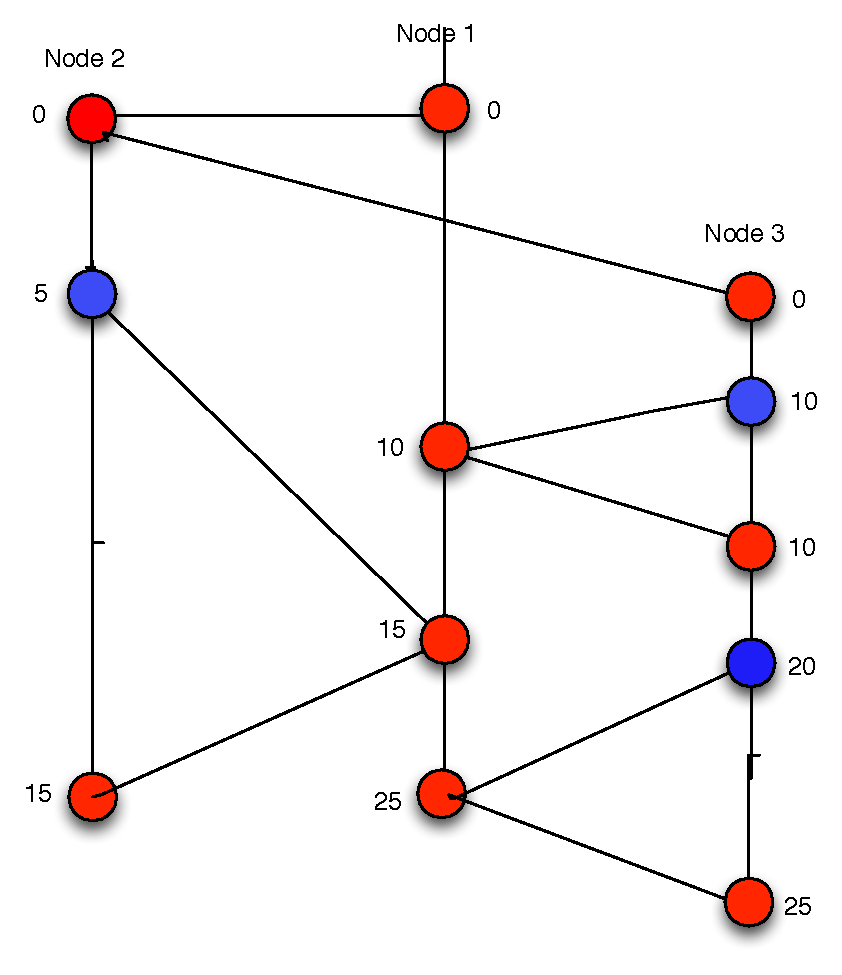
\includegraphics[scale=0.4]{Figures/dali-counter}
  \end{center}
  \caption{\small A replicated counter can be expressed as a sequence
    of versions managed by logically-distributed concurrently
    executing threads.  Local versions produced by these threads
    periodically merge their state with one another.  In the figure,
    when the local version of Node 3, labeled 20, merges with the
    local version of Node 1, whose counter state is 15 at the time, a
    new counter value is produced.  This value takes into account the
    previous merged state (10) from which the two versions were
    derived to yield a new merged state of 25.  There is no other form
    of synchronization or coordination among versions except through
    merging.  In the figure, red circles represent counter state
    produced through merging, and blue circles represent state
    produced by applying counter operations on a node-local version.
  }
\vspace*{-.85in}
\end{wrapfigure}
witness the increment to $c_1$, but not $c_2$, thus violating the
invariant. The intention to atomically apply both effects cannot be
captured in the absence of external mechanisms to compose effects
(such as effect-based transactions~\cite{pldi15}).  Rather than
viewing a distributed computation in terms of \C{Add} effects produced
by operations, can we formulate a more declarative interpretation,
directly in terms of the counter value maintained by each node.  In
doing so, we observe that each replica essentially operates over its
own version of a counter.  Local operations on a replicated object can
be thought of as yielding new versions, thus producing a version tree,
with one branch for each replica.  Thus, every branch represents
different (immutable) versions maintained by different nodes, with the
state produced by the computation performed over a counter on a node
recorded along the node's local branch for the counter.  Now, to
generate a globally consistent view of a counter, we only need to
define a merge operation that explains how to combine two local
versions to produce a new version that reflects both their states.

Framing replication as merging leads to a counter implementation that
bears strong similarity to the original sequential one:
  \begin{ocaml}
    module Replicated_Counter = struct
      include Counter
      let merge lca v1 v2 =
         lca + (v1 - lca) + (v2 - lca)
    end
  \end{ocaml}
The role of \C{lca} (least common ancestor) here captures salient
history - the state resulting from the merge of two versions derived
from the same ancestor state should not unwittingly duplicate the
contributions of the ancestor.  This interpretation of a replicated
datatype is thus given in terms of the evolution of a program state
impicitly associated with the different nodes that comprise a
distributed application with merge operations serving to communicate
and reconcile different local states.

In this paper, we develop a programming model that realizes a monadic
version control system centered around data, rather than file,
coherence.  The \name monad lets programmers write and compose
concurrent computations around multiple (implicit) versions of a
mergeable datatype, an ordinary ML datatype additionally equipped with
a \emph{merge} function responsible for deriving a consistent global
state from a collection of local versions of that state.  A
computation progresses by forking (i.e., replicating) new versions of
existing versions on geo-distributed nodes, allowing
synchronization-free local computation to proceed on those nodes,
creating new versions along an existing \emph{branch} that represents
updated local instances, and by merging branches to realize global
consistency.

Our model allows ML programmers to get the benefits of achieving
highly available (low-latency) distributed computation, while
continuing to enjoy the comforts of high-level reasoning and the
familiarity of using standard libraries already provided by the
language.  Notably, while \name's programming model makes no explicit
reference to any specific operational manifestation of a distributed
system (e.g., programmers do not need to explicitly manage replicas),
we demonstrate that it can be nonetheless efficiently realized on
existing geo-replicated distributed systems.

Our contributions are summarized below:

\begin{itemize}
    \item We formally introduce the concept of a \emph{mergeable}
      datatype to admit high-level declarative reasoning about
      distributed computation and replicated state in ML programs.

    \item We describe \name programming model that brings to bear the
      power and flexibility of a version control system to the
      administration of replicated data. \name hides the complexity of
      version control behind a monad, and exposes its functionality
      via a simple API that lets programmers define and compose
      distributed ML computations around such data.  Issues related to
      replication only manifest implicitly in the definition of a
      merge operation that defines coherence among different instances
      of replicated state.

    \item We present a formalization of the \name programming model,
      and establish the comditions under which eventual convergence of
      concurrent version state can be guaranteed.

    \item We describe an implementation of the \name library that
      transparently adds persistence and replication features to a
      mergeable type, and which sits atop the Irmin persistent
      store~\cite{irmin}, a content-addressable storage library for
      OCaml. We also present case studies and experimental results
      that justify the practical utility of our approach.
\end{itemize}

The remainder of the paper is organized as follows.  We present the
\name\ programming model informally in the next section.
Sec.~\ref{sec:mergeable_types} develops a series of examples that
illustrate how merge operations can be defined and used.
Sec.~\ref{sec:formalization} defines an operational semantics, and
formalizes our intution of a mergeable type in terms of morphisms over
datatype operations.  We also present soundness (consistency) and
progress guarantees enjoyed by the
semantics. Sec.~\ref{sec:system-model} considers an instantiation of
the model suitable for distributed environments with network
partitions and failures.  Implementation details describing how we
incorporate mergeable types into OCaml are presented in
Sec.~\ref{sec:impl}.  Experimental results and benchmarks are given
in Sec.~\ref{sec:evaluation}.



, along with
a series of examples illustrating how merge operations can be defined
and used.  Sec.~\ref{sec:


%% Persistence adds yet another dimension to the problem. Functional data
%% structures are often large in-memory linked structures that admit
%% functional updates by creating newer versions that share most of their
%% structure with previous versions. Sharing is the key to efficiency,
%% without which every functional update takes time that is at least
%% linear in the size of the data structure. Unfortunately, the
%% straightforward way to persist a data structure on disk in a
%% machine-agnostic format (e.g., JSON) requires serialization, which is
%% linear in the size of the data structure. An alternative is to
%% maintain a separate on-disk copy of the data and administer it via a
%% database system. The downside is that the programmer is now required
%% to reason in terms of a lower-level abstraction (e.g., a relational
%% data model) in order to maintain coherence between in-memory and
%% on-disk representations. Safety guarantees over the in-memory data do
%% not carry over to the disk, which introduces additional complications
%% and the possibility of new bugs. Thus, adding persistence to
%% applications while preserving high-level safety gurantees offered by
%% the language abstraction is a non-trivial problem.



%% However, as we shall see,
%% unconstrained branching may yield a branching structure that becomes
%% unmergeable, thus leading to \emph{stuck} states. An important
%% property of the \name library is that it guarantees progress even in
%% the presence of arbitrary merges provided the merge operation is
%% commutative with respect to its version state arguments.  Furthermore,
%% \name profitably exploits provenance information available via
%% branches to make application resilient to network partitions.
%% In this paper, we define a semantics of mergeable datatypes that lets
%% any OCaml program be seamlessly deployed in a distributed environment
%% with implicit support for replicated and decentralized operation.  The
%% underlying foundation for merge actions has a natural category
%% theoretic interpretation that enables us to construct useful mergeable
%% variants for \emph{any} OCaml type whose states are commutative wtih
%% respect to the merge operation defie


% \section{Motivation}

In this section, we motivate mergeable data types and \name
programming model via a series of examples. 

\subsection{Counter}

\begin{figure}

\begin{subfigure}[b]{0.4\textwidth}
  \begin{ocaml}
    module Counter: sig
      type t
      val add: int -> t -> t
      val mult: int -> t -> t
      val read: t -> int
    end = struct
      type t = int
      let add x v = v + (abs x)
      let mult x v = v * (abs x)
      let read v = v
    end
  \end{ocaml}

\caption{\C{Counter} library in OCaml}
\label{fig:counter-adt}
\end{subfigure}
\begin{subfigure}[b]{0.56\textwidth}
  \begin{ocaml}
    module Counter: sig
      type t
      type eff 
      val add: int -> t-> eff
      val mult: int -> t -> eff
      val apply: eff -> t -> t
      val read: t -> int
    end = struct
      type t = int
      type eff = Add of int
      let add x v = Add (abs x)
      let mult x v = Add (v * (abs x - 1))
      let apply (Add x) v = x + v
      let read v = v
    end
  \end{ocaml}

\caption{\C{Counter} library re-engineered for effect-based replication}
\label{fig:counter-rdt}
\end{subfigure}
% \begin{minipage}{0.62\textwidth}
%   \begin{ocaml}
%     module Counter = struct
%       include Counter
%       type t = counter [@@deriving persistence]
%       let merge old v1 v2 = old + (v1 - old) 
%                                 + (v2 - old)
%     end
%   \end{ocaml}
% \end{minipage}

% \caption{\C{Counter} library in OCaml equipped with a \C{merge}
% function. The \C{deriving} syntax~\cite{ppx-deriving} is processed by
% \name's meta-programming library to automatically derive a persistent
% variant of the \C{Counter}}

% \label{fig:counter}
\end{figure}

We will start with a simple example of a counter that nonetheless
demonstrates the benefits of our approach. An OCaml implementation of
the \C{Counter} library is shown in Fig.~\ref{fig:counter-adt}.
\C{Counter} supports two (update) operations - \C{add} and \C{mult} -
that let a non-negative integer value to be added to the counter, and
multiply the counter, respectively. Observe that the library is
written in an idiomatic style in OCaml; any OCaml programmer faced
with the task of implementing the counting functionality would
presumably write the same.  

The counter implementation of Fig.~\ref{fig:counter-adt} serves the
application well as long as it is used in-memory on a single machine.
However, as the application grows in complexity and scales beyond a
single machine, its state may also need to be replicated and
persisted. Unfortunately, replication doesn't come for free, and
existing techniques require significant re-engineering of the
application and its libraries to support replication. A method often
adopted~\cite{crdts, pldi15, gotsman-popl16} is to re-define the operations to
return \emph{effects} instead of values.  An \emph{effect} is a tag that
identifies the operation to be applied uniformly at all
replicas to incorporate the effects of the original operaton. For
instance, \C{Counter.add x v} operation returns \C{Add x} effect,
which, when applied at a replica (see \C{apply}), adds \C{x} to the 
local counter value.  Fig.~\ref{fig:counter-rdt} shows the
\C{Counter} library with operations re-defined to returns effects.
Such re-engineering has to be done carefully, lest an operation may
may end up causing an unintended effect at a remote replica. For
instance, one may incorrectly define \C{mult x v} operation as
generating a \C{Mult x} effect, for it is easy to overlook the fact
that \C{apply (Mult x)} affects different replicas differently
depending on the counter value. Thus, reasoning about the correctness
of effects often involves appeals to system-specific artifacts, such
as replicas, which don't normally manifest in the program.  While
checking the effects (or rather their application via \C{apply}) for
commutativity may help catch some of these oversights, commutativity
is a non-local property, and automatically verifying it is difficult.
Besides introducing the possibility of new bugs, re-engineering
libraries to return effects has obvious software engineering problems
in the sense that it breaks backwards compatibility with the existing
code.

Another downside with effect-generating replicated data type libraries
is that they don't compose. For instance, let us say that an
application wants to use two replicated counters, $c_1$ and $c_2$,
bound by an invariant $c_2 \ge c_1$, which the application duly
enforces when updating $c_2$ and $c_1$. Nonetheless, it may still
witness anamolous states that violate the invariant because updates to
$c_1$ and $c_2$ are applied independently in any order. For example,
if a replica increments both the counters by 1 each, the \C{read} at
another replica, where $(c_1,c_2) = (2,2)$ may witness the increment
to $c_1$, but not $c_2$, thus violating the invariant. The intention
to atomically apply both the effects cannot be captured in the absence
of external mechanisms to compose effects (such as effect-based
transactions~\cite{pldi15}).  

Persistence adds another dimension to the problem. Functional data
structures are often large in-memory linked structures that admit
functional updates by creating newer versions that share most of their
structure with previous versions. Sharing is the key to efficiency,
without which every functional update takes time that is at least
linear in the size of the data structure. Unfortunately, the
straightforward way to persist a data structure on disk in a
machine-agnostic format (e.g., JSON) requires serialization, which is
linear in the size of the data structure. An alternative is to
maintain a separate on-disk copy of the data and administer it via a
database system. The downside is that the programmer is now required
to reason in terms of a lower-level abstraction (e.g., a relational
data model) in order to maintain coherence between in-memory and
on-disk representations. Safety guarantees over the in-memory data do
not carry over to the disk, which introduces additional complications
and the possibility of new bugs. Thus, adding persistence to
applications while preserving high-level safety gurantees offered by
the language abstraction is a non-trivial problem.

\name lets programmers add replication and persistence to their
applications without having to re-engineer their abstractions or
reason about lower-level artifacts. Here is how you write a mergeable
counter in \name:
\begin{figure}[!h]
  \begin{ocaml}
    module Counter = struct
      include Counter
      type mergeable_t = t [@@deriving persistence]
      let merge old v1 v2 = old + (v1 - old) + (v2 - old)
    end
  \end{ocaml}
\end{figure}




%\section{Operational Semantics}

\begin{figure*}[!t]
\raggedright
%
\textbf{Syntax}\\
%
\begin{smathpar}
\renewcommand{\arraystretch}{1.2}
\begin{array}{lclcl}
\multicolumn{5}{c} {
  t \in \mathtt{Thread\; Ids} \qquad
  x,y \in \mathtt{Variables} \qquad
  c \in \mathtt{\{()\}} \cup \mathbb{N} \qquad
}\\
v & \in & \mathtt{Values} & \coloneqq & c \ALT \lambda x.\,s\\
s & \in & \mathtt{Expressions} & \coloneqq & v \ALT s\;s \ALT \run{s}{s}
   \ALT \fork{s} \ALT \pull \ALT \push{s}\\
p & \in & \mathtt{Programs} & \coloneqq & s_t \ALT p\,||\,p \\
f & \in & \mathtt{Tags} & \coloneqq & \C{INIT} \ALT \C{FORK} \;b 
  \ALT \C{PUSH} \ALT \C{MERGE} \;b\\
b & \in & \mathtt{Branches} & \coloneqq & [(v,f)] \ALT (v,f)::b \\
\end{array}
\end{smathpar}
%
\bigskip
%% If we are feeling adventurous, we can try defining e and s 
%% mutually recursively, such that their evaluation relations 
%% are also mutually recursive (multiple reduction steps of one 
%% relation is a single step of other). 

%
\textbf{Evaluation Contexts}\\
%
\begin{smathpar}
\renewcommand{\arraystretch}{1.2}
\begin{array}{lclcl}
H & \in & \mathtt{Branch\; Histories} & \coloneqq & t \mapsto b\\
E & \in & \mathtt{Eval.\; Contexts}(s) & \coloneqq & \bullet \ALT 
  \bullet\;s \ALT v\;\bullet \ALT \run{\bullet}{s}\\
P & \in & \mathtt{Eval.\; Contexts}(p) & \coloneqq & E_t \ALT 
  \bullet\,||\,p \ALT p\,||\,\bullet \\
\end{array}
\end{smathpar}
%
\bigskip

%
\textbf{Reduction Relation} \quad \fbox {$p;\;H \stepsto p';\;H'$} \\
%
%
\begin{smathpar}
\begin{array}{lcll}
(\run{v}{s})_t;\cdot & \stepsto & 
  s_t; \cdot[t_{\top} \mapsto [(v,\C{INIT})]]
            [t\mapsto [(v,\C{FORK}\; [(v,\C{INIT})])]] 
            & [\rulelabel{E-Run}]\\
(\fork{s})_t;H(t\mapsto (v,\_)::b) & \stepsto & 
    ()_t\,||\, s_{t'}; H[t'\mapsto [(v, \C{FORK} H(t))]] 
    \spc \texttt{where}\; t'\not\in dom(H)
            & [\rulelabel{E-Fork}]\\
(\push{v})_t;H & \stepsto & ()_t;H[t \mapsto (v,\C{PUSH})::H(t)]
            & [\rulelabel{E-Push}]\\
% & & & v\,=\,\C{merge}\,v\,v_1\,v_2 ~\texttt{and}~ \\
((\lambda x.s)\;v)_t;H & \stepsto & ([v/x]\,s)_t;H
            & [\rulelabel{E-App}]\\
(\pull)_t;H(t \mapsto (v,\_)::m) & \stepsto & v_t;H
            & [\rulelabel{E-Pull}]\\
\end{array}
\end{smathpar}
%

% %
% \hspace*{\fill}[\rulelabel{E-Admin}]\hspace*{0.25in}
% \begin{smathpar}
% \begin{array}{c}
% \RULE
% {
%   s_t; H ~\stepsto^{*}~ v_t; H
% }
% {
%   E_t[s]; H ~\stepsto^{*}~ E_t[v]; H
% }
% \end{array}
% \end{smathpar}
% %

%
\hspace*{\fill}[\rulelabel{E-Pull-Wait}]
\begin{smathpar}
\begin{array}{c}
\RULE
{
  t\neq t' \spc
  \under{H}{v' \mbleto v} \spc
% \C{world}(H,t') \semsucceq \C{world}(H,t)\spc 
  v_m = \C{merge}(\C{lca}(H(t),H(t')), v, v') \spc
}
{
  (\pull)_t;H(t \mapsto (v,f)::m)(t' \mapsto (v',\_)::\_) ~\stepsto~
  (\pull)_t;H[t \mapsto (v_m,\C{MERGE}\; H(t'))::(v,f)::m]
}
\end{array}
\end{smathpar}
%

\caption{\name: Syntax and Operational Semantics}
\label{fig:opsem}
\end{figure*}


We formalize our ideas in the context of a lambda calculus ($\lang$)
shown in Fig.~\ref{fig:opsem}. Expressions of $\lang$ are variables,
constants, and \name primitives composed using the lambda combinator.
For brevity, we use short names for \name primitives: \C{run} for
\C{with\_init\_version\_do}, and \C{fork} for \C{fork\_version}. To
simplify the technical development, \name's \C{sync\_next\_version}
operation is broken down into two primitives - \C{push} and \C{pull},
which can be lambda-composed get the desired effect:
\begin{smathpar}
  \C{sync}\;x \;=\; (\lambda y.\pull)\; (\push\,x)
\end{smathpar}
The semantics of\C{get\_current\_version} is subsumed by \C{pull},
hence elided.  Values ($v$) are constants and lambda abstractions.  A
program ($p$) is a parallel composition of threads, where each thread
is an expression ($s$) indexed by the corresponding thread identifier
($t$). 

Fig.~\ref{fig:opsem} also shows the syntax of \emph{branches}, which
are the artifacts of evaluation and only appear during the run-time. A
branch is a non-empty sequence of tagged values, where the tag
captures the abstract run-time operation that led to the creation of
the value. It is implicitly assumed that each value added to a branch
is uniquely identifiably, hence no two values on a branch are equal.
The uniqueness assumption is later extended to a collection of
branches that constitute a branching structure. A real implementation
meets this assumption by versioning values across the branches. Thus,
in reality, branches contain \emph{versions} which denote values. The
semantics, however, doesn't make this distinction, and uses values and
versions interchangeably.

Small-step operational semantics of $\lang$ is defined via reduction
relation ($\stepsto$) that relates \emph{program states}. A program
state ($p;\,H$) consists of a program $p$ and a \emph{branch history}
$H$ that maps thread Ids to corresponding branches; each thread is
associated with a branch during the evaluation. Evaluation contexts
have been defined separately for expressions ($E$) and programs ($P$),
with the latter subsuming the former. $E$ is defined to evaluate the
first argument of a \C{run} expression to a value that constitutes the
initial version (recall that \C{run} models \name's
\C{with\_init\_version\_do}). Program evaluation context
non-deterministically picks one of the threads to evaluate. The admin
rule that relates transitions of holes to transitions of expressions
and programs is straightforward, hence elided. Rest of the reduction
rules are presented in Fig.~\ref{fig:opsem}. For brevity, we write
$H(t\mapsto (v,f))$ to denote the proposition that $H$ maps $t$ to
$(v,f)$. The notation $H[t \mapsto (v,f)]$ as usual denotes
the extension of $H$ with the binding $t \mapsto (v,f)$.

Reduction rules let expression evaluation take a step by rewriting the
expression and suitably updating the branch history ($H$). The
\rulelabel{E-Run} rule is applicable only when $H$ is empty, i.e.,
when no prior branching structure exists. The rule rewrites the
$\C{run}\;v\;s$ expression to $s$, while creating a new branching
structure with two branches: a \emph{top} branch that has just the
initial version (tagged with \C{INIT}), and a branch for the current
thread ($t$) forked-off from the top branch.  The first version on the
current branch ($H(t)$) denotes the same value ($v$) as the initial
version on the top branch, although versions themselves are deemed
distinct. The new version is tagged with a \C{FORK} tag that keeps the
record of its orgin, namely the \C{fork} operation and the branch from
which the current branch is forked. The \rulelabel{E-Fork} rule forks
a new thread with a fresh id ($t'$) and adds it to the thread pool.
The corresponding branch ($H(t')$) is forked from the parent thread's
branch ($H(t)$). The semantics of branch forking is same as described
above. The \C{fork} expression in the parent thread evaluates to
\C{()}. The \rulelabel{E-Push} rule creates a new version on the
current branch ($H(t)$) using the pushed value ($v$).
\rulelabel{E-App} is the standard beta reduction rule.

The semantics non-deterministically chooses \rulelabel{E-Pull} or
\rulelabel{E-Pull-Wait} rules to reduce a \C{pull} expression. The
\rulelabel{E-Pull} rule reduces \C{pull} to \C{()}, and returns the
latest version on the current branch. The \rulelabel{E-Pull-Wait} rule
can be thought of as a stutter step; it doesn't reduce \C{pull}, but
updates the branching structure by merging (the latest version of) a
concurrent branch ($H(t')$) into (the latest version of) the current
branch ($H(t)$), and extending the current branch with the merged
version ($v_m$). The new version is tagged with a \C{MERGE} tag that,
like a \C{FORK} tag, records its origin. The premises of the
\rulelabel{E-Pull-Wait} serve the important purpose of contraining the
branching structure by allowing only the legal merges, and
consequently preserving certain desirable properties of the system;
we will go into the details shortly. The \rulelabel{E-Pull-Wait} and
\rulelabel{E-Pull} rules thus let a thread sync with a subset of
concurrent threads in multiple steps before returning the result of
the \C{pull}. Since \C{sync} is a composition of \C{push} and
\C{pull}, its behavior can be explained thus: \C{sync} pushes the
given value onto the current (local) branch, merges a (possibly empty)
subset of concurrent branches into the local branch, and returns the
result.

We will now present a series of definitions and results that let us
understand the premises of the \rulelabel{E-Pull-Wait} rule, examine
the merge operation in closer detail, and appreciate the need for
constraining the branching structure. First, we formalize the
intuitive notation of the ancestor relationship between versions of a
legal branching history (i.e., a branching history generated by the
rules in Fig.~\ref{fig:opsem}):

\begin{definition} [\bfseries Ancestor]
Version $v_1$ is a ancestor of version $v_2$ under a history
$H$ (written $\under{H}{v_1 \preceq v_2}$) if and only if one of the
following is true:
\begin{itemize}
  \item There exists a branch $b$ in $H$ (i.e., $\exists(t\in
  dom(H)).\,H(t) = b$) in which $v_2$ immediately succeeds
  $v_1$,
  \item There exists a branch $b$ in $H$ that contains $(v_2, 
  \C{FORK}\; (v_1,f_1)::b_1)$, for some $f_1$ and $b_1$,
  \item There exists a branch $b$ in $H$ that contains
  $(v_2, \C{MERGE}\;(v_1,f_1)::b_1)$, for some $f_1$ and $b_1$,
  \item $v_1 = v_2$, or $v_1$ is transitively a ancestor of
  $v_2$, i.e., $\exists v.~ \under{H}{v_1 \preceq v} \conj
  \under{H}{v \preceq v}$ 
\end{itemize}
\end{definition}

Ancestor relation is therefore a partial order (reflexive, transitive,
anti-symmetric) with a greatest lower bound (the initial version).
Thus, for any two versions in a legal history, there exist at least
one common ancestor. Ancestor relationships among the common ancestors
let us define the notion of a least common ancestor (LCA):

\begin{definition} [\bfseries Least Common Ancestor]
Version $v$ is said to be a common ancestor of versions $v_1$ and
$v_2$ under a history $H$ if and only if $\under{H}{v \preceq v_1}$
and $\under{H}{v \preceq v_2}$. It is said to be the least common
ancestor (LCA) of $v_1$ and $v_2$, iff there does not exist a $v'$
such that $\under{H}{v' \preceq v_1}$ and $\under{H}{v' \preceq v_2}$
and $\under{H}{v \preceq v'}$.
\end{definition}

\begin{figure}
\centering
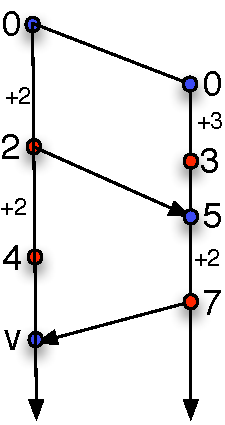
\includegraphics[scale=0.6]{Figures/merge-needs-lca}

\caption{This example of a grow-only counter illustrate why \C{merge}
needs a least common ancestor, and not just a common ancestor. Both 0
and 2 are common ancestors of 4 and 7, while 2 is their least common
ancestor (since $0 \preceq 2$). The result (v) of merging 4 and 7 is
11 (incorrect) if 0 is used as the common ancestor for merge, and 9
(correct, because 2+2+3+2 = 9) if 2 is used. }
\label{fig:merge-needs-lca}
\end{figure}

\begin{figure}[!t]
\centering
\subcaptionbox[] {\small
  In this example, 1 and 3 have two LCAs (3 and 4) a result of
  previous merges. The dotted circle denotes a virtual ancestor
  obtained by merging the two LCAs.
  \label{fig:criss-cross-lcas}
} [0.47\columnwidth] {
  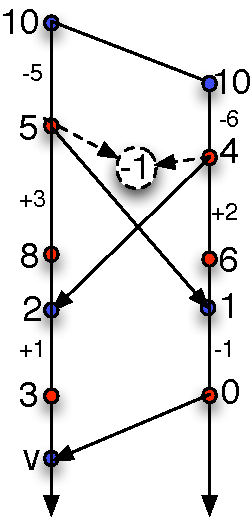
\includegraphics[scale=0.55]{Figures/2-LCAs}
}
\hfill
\subcaptionbox[] {\small
  In this example, 3 and 6 have two LCAs (2 and 1) despite there not
  being any previous merges between their respective branches.
  \label{fig:external-lcas}
} [0.47\columnwidth] {
  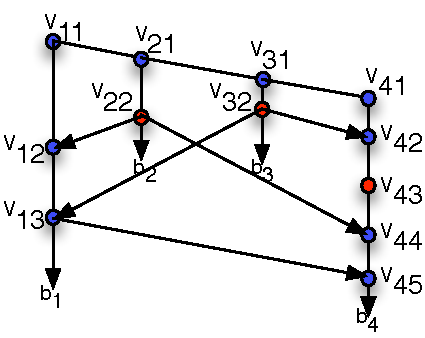
\includegraphics[scale=0.7]{Figures/2-external-LCAs}
}
\caption{Examples where merging versions have more than one LCA}
\label{fig:many-lcas}
\end{figure}

When merging two concurrent versions $v_1$ and $v_2$, the common
ancestor argument for \C{merge} must the LCA of $v_1$ and $v_2$,
without which \C{merge} may yeild unexpected results. This is
demonstrated for the grow-only counter in
Fig.~\ref{fig:merge-needs-lca}, where incorrect count is obtained if a
common ancestor that is not an LCA is used to merge 4 and 7. While in
this example there is a unique LCA for 4 and 7, in general this may
not be the case. With unrestrained branching and merging, there is no
bound on the number of LCAs a pair of versions can have.
For example, in
Fig.~\ref{fig:criss-cross-lcas}, the merge of 0 with 3 is preceded by
two ``criss-cross'' merges between their respective branches resulting
in there being two LCAs (5 and 4) for 0 and 3. Multiple LCAs can occur
even without criss-cross merges, as demonstrated by
Fig.~\ref{fig:external-lcas}. The problem with concurrent versions
with multiple LCAs is that they do not lend themselves to three-way
merging. This problem also arises in the context of source
control systems, and often solved via ad-hoc mechanisms.
GitHub~\cite{github}, for instance, recursively merges LCAs to compute
a virtual ancestor, which then serves as the LCA for merging the
concurrent versions. This method is demonstrated for the example in
Fig.~\ref{fig:criss-cross-lcas}, where LCAs 5 and 4 of 0 and 3 are
merged (with LCA of 10) to generate -1 as the virtual LCA to merge 5
and 4. A major downside with this method is that it makes no
guarantees of the relationship between the virtual ancestor and the
concurrent versions; the former may not even be a legal ancestor of
the latter as per the semantics of the data type. For instance, the
integer type in Fig.~\ref{fig:criss-cross-lcas} may in fact represent
a bank account, which disallows any activity on the account if balance
is ever known to be less than zero. Thus, from the perspective of a
bank account, it doesn't make sense how concurrent versions 3 and 0
emerged from -1, since the only transition allowed by the semantics
from -1 is to itself. Clearly, ad hoc mechanisms, which work for the
text, may not work for more sophisticated data types.

Fortunately, unlike the source control systems where branching
structure is entirely dictated by the user, \name abstracts away the
branching structure from the programmer, hence retains the ability to
constrain it in a way that it deems fit. In particular, \name solves
the problem of multiple LCAs by suitably constraining the branching
structure such that the problem never arises. The constraints are
imposed either implicitly, as a result of how operational semantics
defines an atomic step, or explicitly, by insisting that certain
conditions be met before merging a pair of versions
(\rulelabel{E-Pull-Wait}). Firstly, the operational semantics already
disables criss-cross merges since it only ever merges versions that
are latest on their respective branches. For instance let $v_{11}$ and
$v_{21}$ be the latest versions on branches $b_1$ and $b_2$,
respectively. Meging $b_2$ into $b_1$ requires entails $v_{21}$ into
$v_{11}$ to generate version $v_{12}$ on $b_1$. Now, merging $b_1$
into $b_2$ translates to merging $v_{12}$ into $v_{21}$ (a
\emph{fast-forward} merge, in Git parlance), but not $v_{11}$ into
$v_{21}$, thus preventing a criss-cross branching structure. In other
words, a criss-cross branching structure is prevented due to the
order among merges between conflicting branches introduced as a result
of \rulelabel{E-Pull-Wait} being an atomic step. 

Secondly, we impose certain pre-conditions on the merging branches to
preempt the structure shown in Fig.~\ref{fig:external-lcas}. The
intuition is as follows: consider the branch $b_1$ at the instance of
merging $b_3$. Since it has already merged $b_2$, a version on $b_2$
($v_{22}$) could be a common ancestor for a version on $b_1$
($v_{12}$) and some other version (call it $v$). Now, if $b_1$ merges
$b_3$, same could be true of $b_3$ and $b_1$: a version on $b_3$
($v_{32}$) could be a common ancestor for the new version on $b_1$
($v_{13}$), and the other version $v$. Since $v_{22}$ is also an
ancestor of $v_{13}$, and both ancestors are not ordered by the
ancestor relation, $v_{13}$ and $v$ end up with two LCAs. In
Fig.~\ref{fig:external-lcas}, the role of $v$ is played by the version
$v_{44}$. We observe that this scenario can be prevented if, when
merging $b_3$, $b_1$ insists on an ancestor relation between the
merged version ($v_{22}$) of the $b_2$, the previously merged branch,
and the latest version of $b_3$, the current merging branch. We call
the last merged version the \emph{external locus} of the branch. By
requiring that, for every branch $b$, the external locii of $b$ at
various points in time (i.e., external locus of every prefix of $b$)
be totally ordered, we effectively enforce the invariant that for any
two common ancestors $v_1$ and $v_2$ between two versions, there
exists another common ancestor $v_3$ that succeeds $v_1$ and $v_3$ in
the ancestor relation, thereby preventing the possibility of multiple
LCAs.

%% <false>
%% Multiple versions that merge any pair of versions are totally
%% ordered. That is, if $v_1$ and $v_2$ are ancestors of $v_3$ and
%% $v_4$, then $v_3$ and $v_4$ are ordered by the ancestor relation.
%% </false>

%% If $v_1$ and $v_2$ are ancestors of $v_3$ and $v_4$, then there
%% exists a $v_5$, a successor of $v_1$ and $v_2$, and an ancestor of
%% $v_3$ and $v_4$
%% If I follow one of your locii, or you follow one of my locii, then
%% we both have same set of external common ancestors.

Let us see how the aforementioned restriction allows us to merge the
branches in Fig.~\ref{fig:external-lcas} without ever creating
multiple LCAs. The legal branching history is shown in
Fig.~\ref{fig:legal-merge}. First, like in
Fig.~\ref{fig:external-lcas}, $b_2$ is merged into $b_1$ to create
$v_{12}$, and $b_3$ is merged into $b_4$ to create $v_{42}$. Thus, the
external locus of $b_1$ is $v_{22}$, and that of $b_4$ is $v_{32}$.
Observe that now $b_1$ cannot merge $b_3$, neither can $b_4$ merge
$b_2$ because $v_{22}$ and $v_{32}$ are not related by the ancestor
relation. Same applies for $b_1$ and $b_4$ because neither one's
latest version follows from other's external locus.  However, $b_2$
and $b_3$ can merge among themselves. Let us say they indeed merge to
to create a version $v_{23}$ on $b_2$. The branch $b_2$ is now
eligible to be merged into $b_1$ and also $b_4$. These merges do occur
in Fig.~\ref{fig:legal-merge} to create versions $v_{13}$ and
$v_{43}$, and making $v_{23}$ the external locus for both $b_1$ and
$b_4$. Thus, $b_1$ can now merge into $b_4$ to create version $v_{44}$
on $b_4$.

We now formalize the intuitions described above to precisely define
the notion of mergeability:

\begin{definition} [\bfseries Internal and External Ancestors]
Given a branch $b$ and a version $v\in b$, an internal ancestor of $v$
is an ancestor from the same branch $b$. An external ancestor of $v$
is an ancestor from a different branch $b'\neq b$. 
\end{definition}

\begin{definition} [\bfseries External Locus]
Given a branch $b$ and a version $v\in b$, external locus ($v_o$) of
$v$ is an external ancestor that is not an ancestor of any other
external ancestor of $v$. That is, $\under{H}{v_o \preceq v}$, and
there does not exist a $v_o' \not\in b$ such that $\under{H}{v_o'
\preceq v}$ and $\under{H}{v_o \preceq v_o'}$. 
\end{definition}

\begin{definition} [\bfseries Mergeability]
Given a history $H$, a version $v_1$ and a version $v_2$ that is not
an ancestor of $v_1$ under $H$, $v_2$ is mergeable into $v_1$ (denoted
$\under{H}{v_2 \mbleto v_1}$) iff $v_1$'s external locus is an
ancestor of $v_2$, or $v_2$'s external locus is an ancestor of $v_1$.
\end{definition}

Rule \rulelabel{E-Pull-Wait} of the reduction relation
(Fig.~\ref{fig:opsem}) is enabled only if the latest version ($v'$)
of thread $t'$'s branch is mergeable into the latest version ($v$) of
thread $t$'s branch (i.e., $\under{H}{v' \mbleto v}$). Merge computes
the latest common ancestor of $v$ and $v'$, which is 
guaranteed to be unique as per the following theorem\footnote{Proof
included in the appendix}:

\begin{theorem} [\bfseries Unique LCA]
Every pair of versions $v_1$ and $v_2$ in a legal branch history $H$ 
have a unique least common ancestor. 
\end{theorem}

The \rulelabel{E-Pull-Wait} uses the function \C{lca} to compute the
LCA of (the latest versions on) a pair of branches. The definition of
the function is standard, hence not discussed.


%% Acknowledgments
% \begin{acks}                            %% acks environment is optional
%                                         %% contents suppressed with 'anonymous'
%   %% Commands \grantsponsor{<sponsorID>}{<name>}{<url>} and
%   %% \grantnum[<url>]{<sponsorID>}{<number>} should be used to
%   %% acknowledge financial support and will be used by metadata
%   %% extraction tools.
%   This material is based upon work supported by the
%   \grantsponsor{GS100000001}{National Science
%     Foundation}{http://dx.doi.org/10.13039/100000001} under Grant
%   No.~\grantnum{GS100000001}{nnnnnnn} and Grant
%   No.~\grantnum{GS100000001}{mmmmmmm}.  Any opinions, findings, and
%   conclusions or recommendations expressed in this material are those
%   of the author and do not necessarily reflect the views of the
%   National Science Foundation.
% \end{acks}


%% Bibliography
%\bibliography{bibfile}


%% Appendix
\appendix
\section{Appendix}

Text of appendix \ldots

\end{document}
